% Source for the figure of CircularIterator (sec. 1.8): a circular vector of
% capacity c = 8 whose head is at the place 5, the items v0 .. v4 by their
% index i from the head; *it, with it on i = 2, reads the place 7, and
% it[2] the place (5 + 2 + 2) mod 8 = 1. Build: make figures (in ../build).
\documentclass[border=4pt]{standalone}
\usepackage[T1]{fontenc}
\usepackage{lmodern}
\usepackage{amsmath,amssymb}
\usepackage{tikz}
\usepackage{lamalunga}
% tikz-ads.tex: the TikZ styles shared by the figures of the memory of the
% manual, \input by each standalone figure: a cell of a vector (cell), the
% cell that an operation touches (touched), a free cell (free), a node of a
% linked structure (node), the labels of indices (index) and of variables
% (var), a pointer (ptr), and \cells and \indices to draw a row of cells.
\usetikzlibrary{arrows.meta,positioning,calc,fit,shapes.multipart}
\definecolor{adsTouched}{RGB}{214,196,236}
\definecolor{adsFree}{RGB}{236,236,236}
\tikzset{
  ads/.style={>={Stealth[length=2mm]},font=\small,
              every node/.append style={inner sep=0pt}},
  cell/.style={draw,minimum width=7mm,minimum height=7mm,
               font=\small\ttfamily,outer sep=0pt},
  touched/.style={cell,fill=adsTouched},
  free/.style={cell,fill=adsFree,text=black!45},
  node/.style={draw,rounded corners=1pt,minimum width=8mm,
               minimum height=6mm,font=\small\ttfamily},
  index/.style={font=\scriptsize\ttfamily,text=black!60},
  var/.style={font=\small\itshape},
  ptr/.style={->,thick}
}
% \cells{name}{x,y}{list}: a row of cells, the first at (x,y), named
% name-0, name-1, ...; each item is text/style, the style one of cell,
% touched and free (e.g., {a/cell,e/touched,/free})
\newcommand{\cells}[3]{%
  \foreach \v/\s [count=\i from 0] in {#3}
    \node[\s] (#1-\i) at ($(#2)+(\i*7mm,0)$) {\v};}
% \indices{name}{n}: the indices 0 .. n-1 under the cells of name
\newcommand{\indices}[2]{%
  \foreach \i in {0,...,\numexpr#2-1\relax}
    \node[index,below=1.2mm of #1-\i] {\i};}

\begin{document}
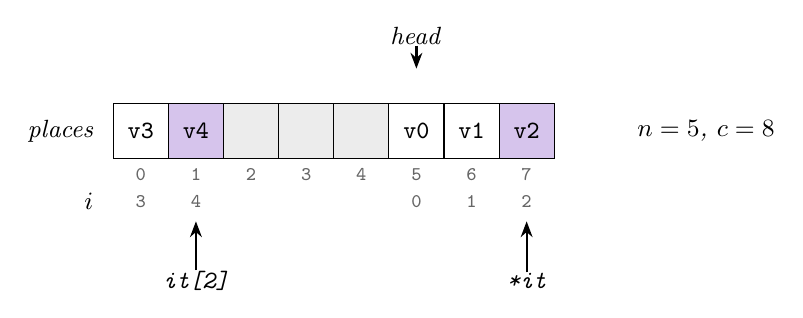
\begin{tikzpicture}[ads]
  \node[var,anchor=east] at (-6mm,0) {places};
  \cells{a}{0,0}{v3/cell,v4/touched,/free,/free,/free,v0/cell,v1/cell,v2/touched}
  \indices{a}{8}
  \node[var,anchor=east] at (-6mm,-9mm) {$i$};
  \foreach \p/\i in {0/3,1/4,5/0,6/1,7/2}
    \node[index] at ($(a-\p)+(0,-9mm)$) {\i};
  \node[var] (it) at ($(a-7)+(0,-19mm)$) {\texttt{*it}};
  \node[var] (ik) at ($(a-1)+(0,-19mm)$) {\texttt{it[2]}};
  \draw[ptr] (it) -- ($(a-7)+(0,-11.5mm)$);
  \draw[ptr] (ik) -- ($(a-1)+(0,-11.5mm)$);
  \node[var] (h) at ($(a-5)+(0,12mm)$) {$\mathit{head}$};
  \draw[ptr] (h) -- ($(a-5.north)+(0,4.4mm)$);
  \node[var,anchor=west] at (63mm,0) {$n = 5$, $c = 8$};
\end{tikzpicture}
\end{document}
